\documentclass[10pt,a4paper]{article}
\usepackage[UTF8]{ctex}
\usepackage{amsmath}
\usepackage{amsfonts}
\usepackage{amssymb}
\usepackage{float}
\usepackage{tikz}           %for TikZ graphics  
\usepackage{tikz-3dplot}
%\usepackage{clrscode}
\usepackage[]{algorithm2e}
\usepackage{listings}
\lstset{
  basicstyle=\small,
  numbers=left,
  keywordstyle=\color{blue},
  numberstyle={\tiny\color{lightgray}},
  stepnumber=1, %行号会逐行往上递增
  numbersep=5pt,
  commentstyle=\small\color{red},
  backgroundcolor=\color[rgb]{0.95,1.0,1.0},
  showspaces=false,
  showtabs=false,
  frame=shadowbox, framexleftmargin=5mm, rulesepcolor=\color{red!20!green!20!blue!20!},
% frame=single,
%  TABframe=single,
  tabsize=4,
  breaklines=tr,
  extendedchars=false %这一条命令可以解决代码跨页时,章节标题,页眉等汉字不显示的问题
}
\usepackage{graphicx}
% Set the margin of document.
\usepackage[top=10mm, bottom=12.5mm, left=12.5mm, right=12.5mm]{geometry}
\usepackage{longtable}
\usepackage{float}
\renewcommand\figurename{图}
\renewcommand\tablename{表}
\title{实验数据的统计处理}
\author{袁略真\\3130103964\\生物信息学\\浙江大学}
\begin{document}
\maketitle
\section{导言}
数据可以来源于实验或计算机计算.数据的分布可有统计直方图展示.

实验得到的数据是有误差的,其中的随机误差导致测量结果的不确定性.期望、方差、标准误差、算术平均值、偏差、标准偏差(贝塞尔公式)、测量值方差,平均值的标准偏差是基本的统计概念.其中,某一物理量的期望、方差和标准误差由于是极限值,因而无法得到.能够得到是后面的一些量.

错误值是在数据采集、传输与记录过程中,由于强干扰或突发性异常的条件变化,或由于一记录介质的故障,或测量实物造成的数据丢失、个别数据的不切实际的偏差.错误值也被称作奇异项或坏值.错误值与误差较大点是性质不同的数据.后者是偶然误差,符合客观,不应被剔除.剔除错误值的目的是恢复数据的客观真实性,而不是为了提高精度.常用的方法如拉依达方法.
\section{程序流程}
\begin{enumerate}
\item 产生随机数,形成数据集(输入N,n,输出data,并输出到文件out(文件名$str,str\_dataset.txt$))
\item 画直方图(输入data,s,输出频数表$str\_freqtable.txt$)
\item 计算基本统计量(输入data,输出平均值avera,平均值的标准偏差avestandevia)
\item 错误值剔除(输入data,输出原始data到文件中,data变量原处修改)
\end{enumerate}
其中N为抽取N个[0,1)随机数,取均值记为几个数据点.n为这样的数据点的总数,数据存储在data变量.s指把[0,1)划分为s个小区间.

\subsection{随机数的产生}
本程序使用C++2011 标准库中$<random>$库.随机数种子由`$std::random\_device$',它产生均匀分布的整数,它本身不是算法产生的,是真随机数,在密码学中有应用.

随机数种子用于初始化伪随机数生成器,在此,我选用`$std::mt19937\_64$',它是`64-bit Mersenne Twister' 法生成的随机数.

生成随机数后,进一步使用`$std::uniform\_real_distribution<double> dr(0,1);$' 获得[0,1)的均匀分布的随机数\footnote{在$<$C++标准库-自学教程与参考手册(Nicolai M.Josuttis)$>$第17.1节中推荐先使用随机数生成器, 再使用分布(`$std::uniform\_real\_distribution<double>$'之类的方法)}.
\subsection{程序架构}
本次作业程序使用C++面向对象的程序设计,将上述程序流程中每一项任务编写成类`SimpleStatisticsProject' 的一个成员函数,它们之间的数据交换通过类的数据成员实现.类的结构如下所示:

\begin{lstlisting}[language=C++]
class SimpleStatisticsProject{
private:
    int m_N,m_n;
    vector<double> m_data;
    ofstream m_out;
    string m_str;
    int m_s;
    double avera,avestandevia;
public:
    SimpleStatisticsProject():m_N(3),m_n(1000),m_data(),m_out(),m_str("result"),m_s(10),avera(0),avestandevia(0){}
    SimpleStatisticsProject(int N,int n,string str,int s):m_N(N),m_n(n),m_data(m_n),m_out(),m_str(str),m_s(s),avera(0),avestandevia(0){}
    ~SimpleStatisticsProject(){}
    void Dataset(int N,int n, string str);//Generate dataset through random numbers. When you want N change and generate new dataset, just call this function!

    void Histogram(int s=10);//get frequancy table
    void Statistic();//calculate average, standard deviation fo average
    void ChangeParameter(int n,int s,string str){m_n=n;m_s=s;m_str=str;}
    void PautaFilter();//pauta criterion
};
\end{lstlisting}
\section{实验结果}
\begin{table}[H]
\centering
\begin{tabular}{|c|c|c|}
\hline 
& N=3&N=10 \\ 
\hline 
平均值&0.505343&0.496856\\
平均值的标准偏差&0.00525362&0.00288611\\
拉依达法错误值数目&0&2(of 1000)\\
\hline
\end{tabular}
\caption{N=3,10时的计算结果.直方图结果见图\ref{fig:1},\ref{fig:2},\ref{fig:3}}
\end{table}

\begin{figure}[H]
\begin{minipage}[b]{0.5\linewidth}
\centering
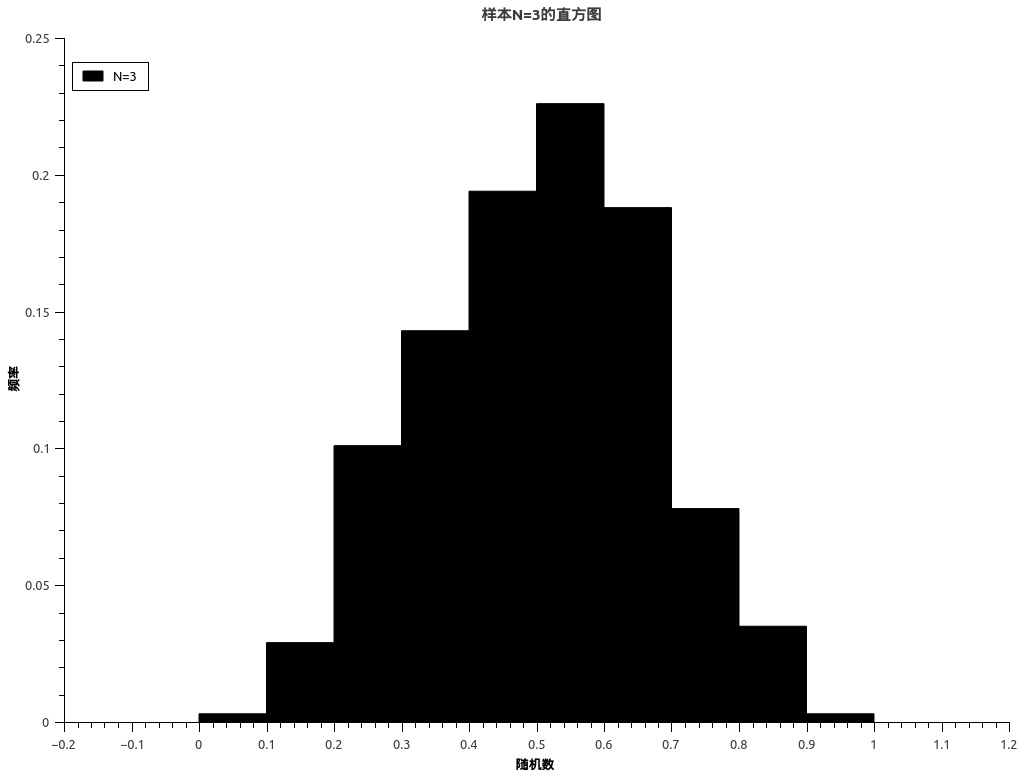
\includegraphics[width=\textwidth]{../result/Table1.png}
\caption{N=3时的直方图.拉依达法没有发现错误值.}
\label{fig:1}
\end{minipage}
\begin{minipage}[b]{0.5\linewidth}
\centering
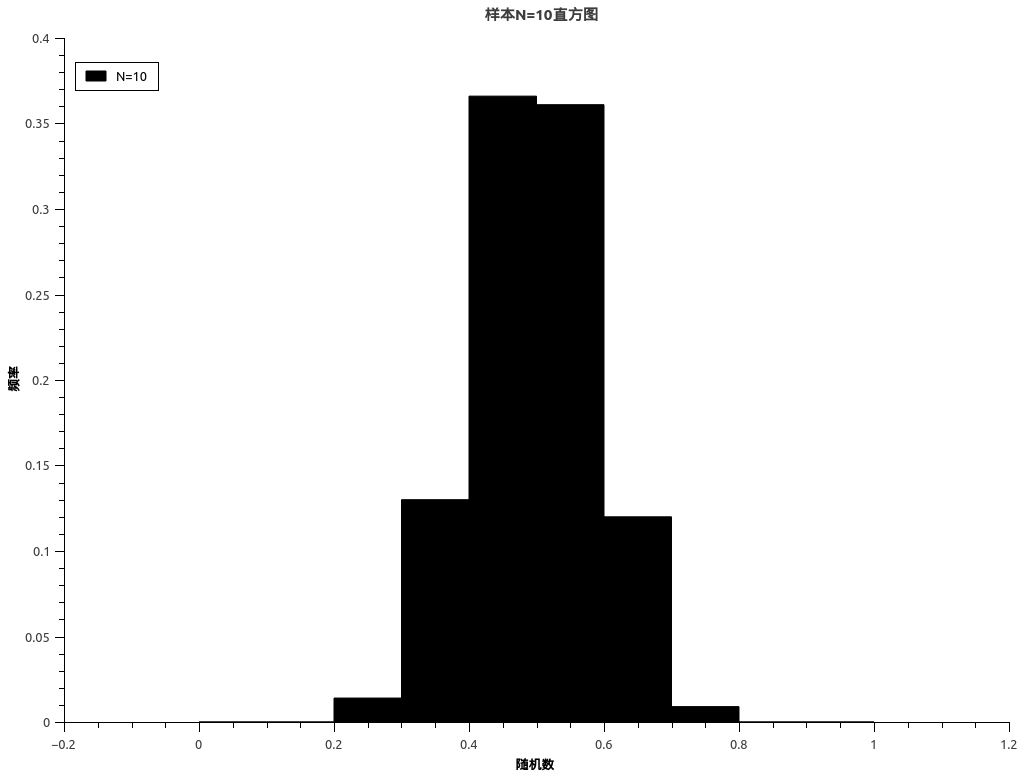
\includegraphics[width=\textwidth]{../result/Table2.png}
\caption{N=10时的直方图.原始直方图.}
\label{fig:2}
\end{minipage}
\begin{minipage}[b]{0.5\linewidth}
\centering
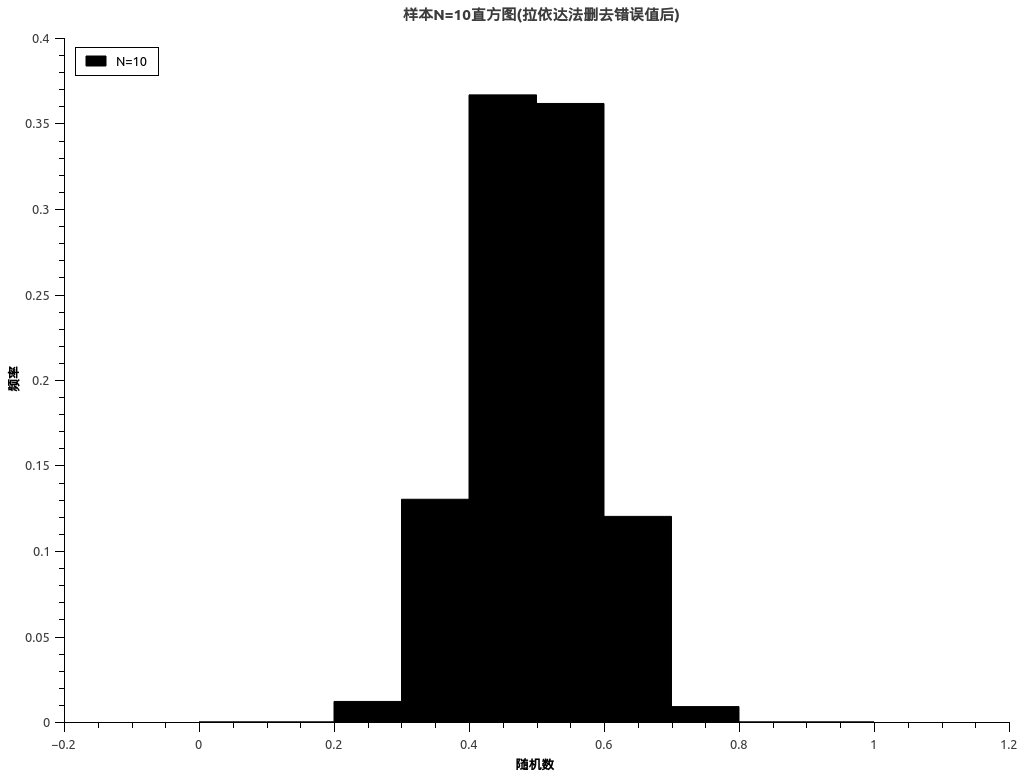
\includegraphics[width=\textwidth]{../result/Table3.png}
\caption{N=10时的直方图.拉依达法去掉两点后的直方图.}
\label{fig:3}
\end{minipage}
\end{figure}
\subsection{$\sigma_{\bar{x} \backsim N}$关系曲线}
\begin{figure}[H]
\centering
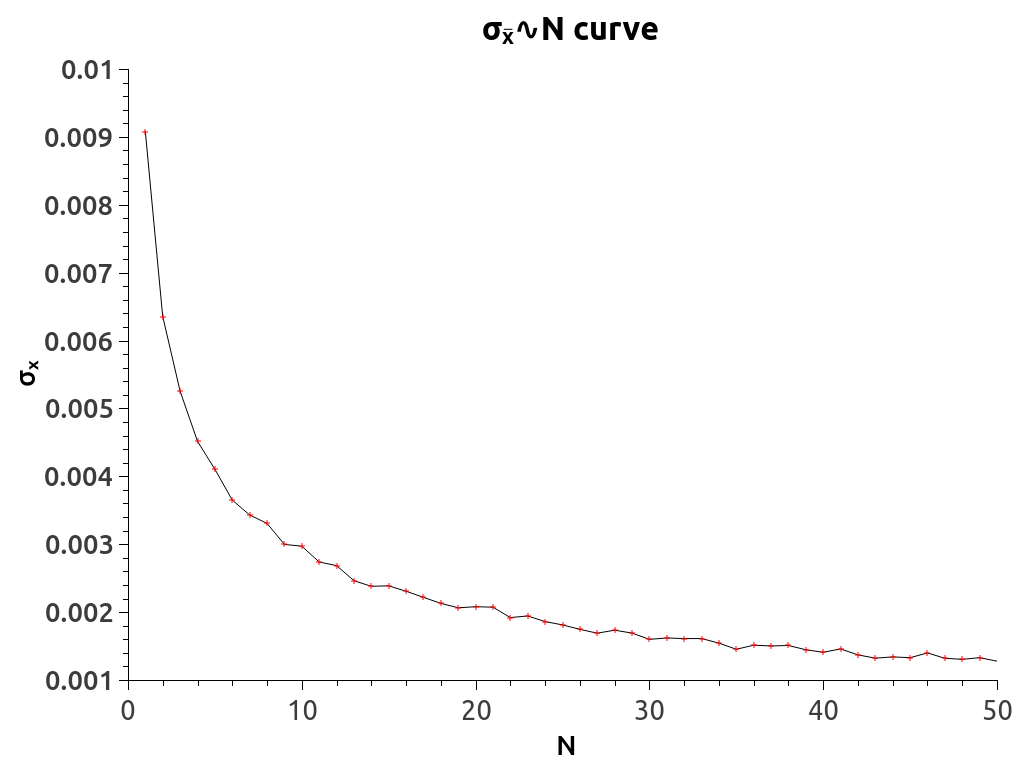
\includegraphics[width=\textwidth]{../result/Graph3.png}
\caption{$\sigma_{\bar{x} \backsim N}$关系曲线.N=1,2,...,50.n=1000,s=10.}
\end{figure}

\end{document}